%!TEX root = ../thesis.tex

\chapter{Методи та підходи вирішення задач класифікації}
\label{chap:review}  %% відмічайте кожен розділ певною міткою -- на неї наприкінці необхідно посилатись

В даному розділі будуть основні теоретичні відомості про об'єкт дослідження та огляд суміжних робіт в даній сфері.

\section{Задача класифікації: визначення, види}

Класифікація -- це процес віднесення об'єкту до певної категорії або класу на основі його характеристик, серед заздалегідь встановленого набору категорій. Класифікація може бути бінарною, багатокласовою, багатомітковою, ієрархічною та інші. Бінарна класифікація -- це класифікація, коли кожному об'єкту обирається група з наперед визначеної множини груп в якій знаходиться рівно дві групи; багатокласова класифікація -- це класифікація, коли кожному об'єкту обирається група з наперед визначеної множини груп в якій може знаходиться довільна кількість груп. В поточній роботі ми зосередимося на бінарній та багатокласовій класифікації.

Задача класифікації зустрічається в багатьох сферах, наприклад: медицина (діагностика раку на основі зображень МРТ), фінанси (класифікація позичальників як \glqq надійних\grqq\ чи \glqq ризикованих\grqq\ на основі їхньої кредитної історії), роздрібна торгівля (класифікація покупців за типами покупок для надання персоналізованих знижок), транспорт (розрізнення між легковими авто, вантажівками та мотоциклами на дорозі), освіта (ідентифікація студентів, яким потрібна додаткова допомога в певних предметах), безпека (класифікація електронних листів як \glqq безпечні,\grqq\ \glqq спам\grqq\ або \glqq фішинг\grqq), біотехнології (розпізнавання мутацій, що спричиняють хвороби). 

\section{Способи вирішення задачі класифікації}\label{sec:methods_of_solving_the_classification_problem}

Існує декілька способів для вирішення задачі класифікації: класичні статистичні методи (наприклад, логістична регресія~\cite{ct1}), алгоритми ML (наприклад, метод k-найближчих сусідів~\cite{ct4}), глибинне навчання (за допомогою нейронних мереж), а також задачу класифікації можна вирішувати за допомогою генетичних алгоритмів.

На початку розглянемо методи глибинного навчання для вирішення задач класифікації. Обчислювальним об'єктом в глибинному навчанні є нейронна мережа. Існують різноманітні типи нейронних мереж, але ми будемо їх розглядати на прикладі MLP~\cite{ct26}, оскільки саме його ми використовуємо для експериментів. MLP~\cite{ct26} складається з шарів нейронів. Кожен нейрон в шарі, приймає вхідні дані з попереднього шару та обчислює вихідний сигнал, який передається наступному шару. Формально штучний нейрон можна описати наступним чином:
\begin{equation}
\label{eq:neuron}
	a = f\left(\sum_{i=1}^n w_i x_i + b \right)
\end{equation}
де \(x_1, x_2, \ldots, x_n\) — вхідні сигнали до нейрону; \(w_1, w_2, \ldots, w_n\) — ваги, що призначені для кожного вхідного сигналу; \(b\) — зсув (англ. bias), що додається до суми зважених вхідних сигналів; \(f\) — активаційна функція, яка має наступні властивості: нелінійність, дииференційовність, неперервність, монотонність. 

В нейронній мережі може бути довільна кількість шарів та в кожному шарі може бути довільна кількість нейронів. Усі вони працюють за вище наведеним принципом: на вхід кожному нейрону в кожному шарі приходить сигнал з попереднього шару і кожний нейрон генерує вихід, якщо це перший шар, то на вхід подаються самі дані. Загалом схема нейронної мережі може виглядати наступним чином (рисунок \ref{fig_nn_arch}).

\begin{figure}[ht]
	\centering
	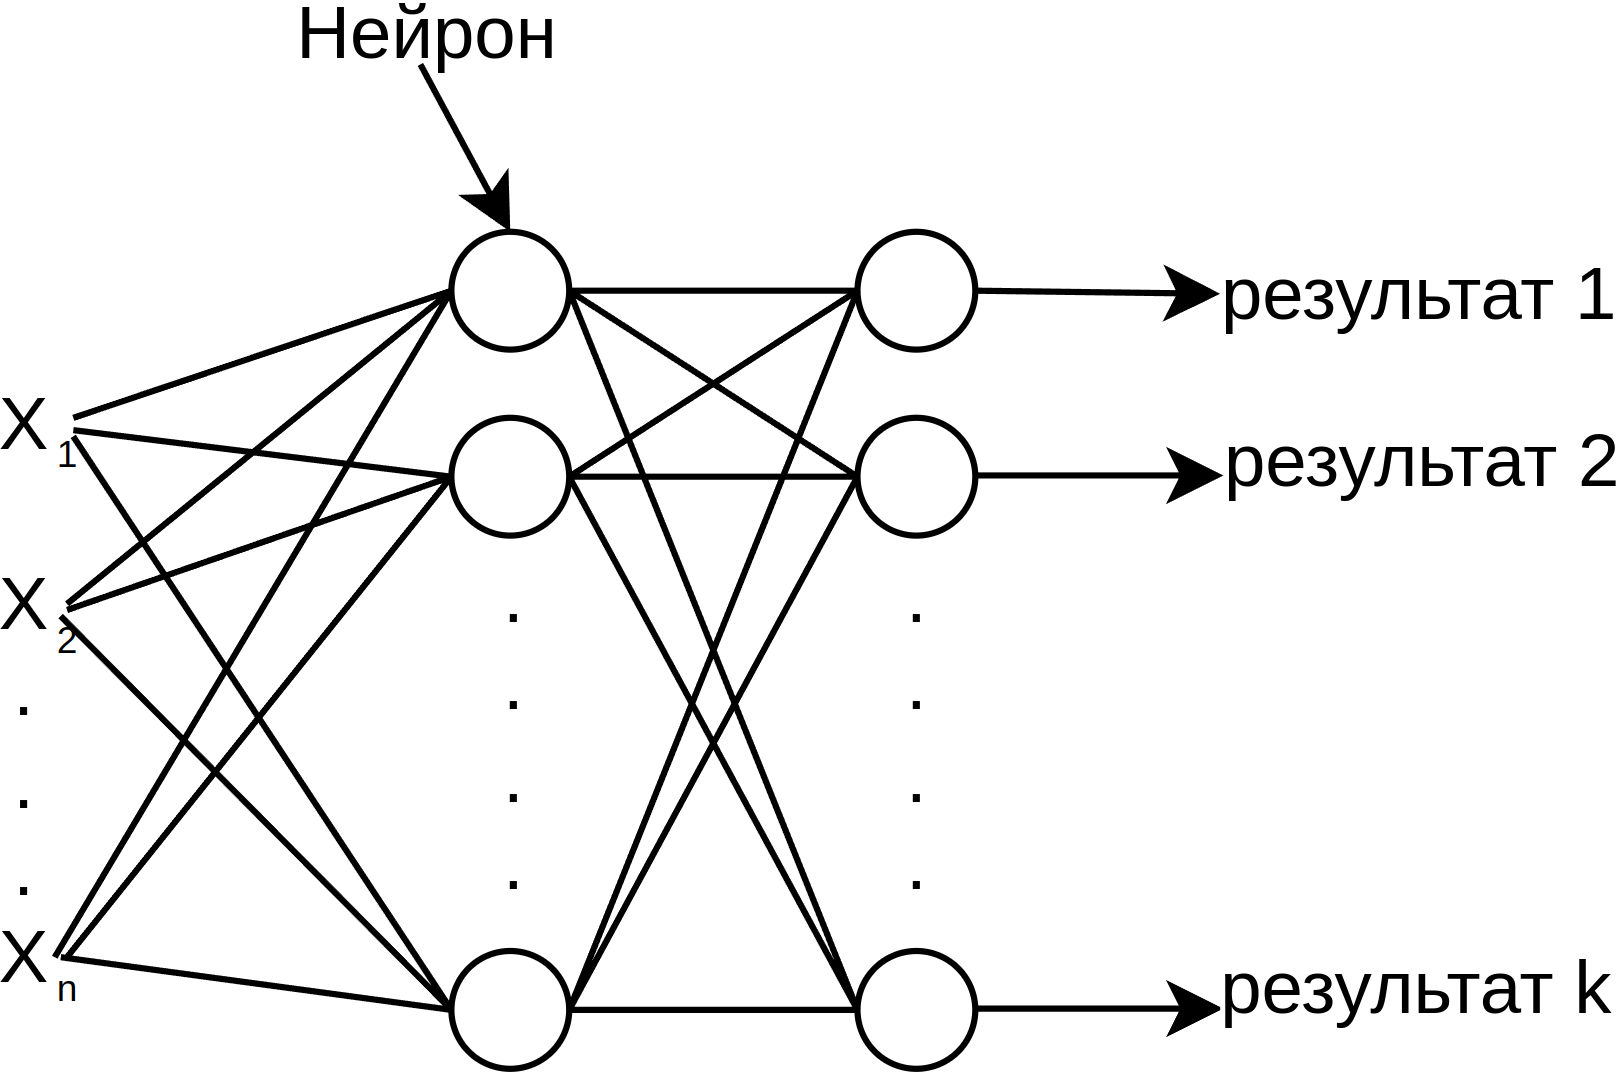
\includegraphics[scale=0.5]{Images/neural_network_architecture.png}
	\caption{Загальна архітектура повнозв'язної нейронної мережі}
	\label{fig_nn_arch}
\end{figure}

Далі розглянемо генетичні алгоритми для вирішення задач класифікації. Обчислювальним об'єктом в генетичних алгоритмах є індивід (див. означення в переліку умовних позначень, скорочень і термінів). Індивід може бути представлений різними способами, але ми будемо розглядати представлення, яке найчастіше використовується в GP, а саме -- дерево (приклад дерева -- рисунок \ref{fig_genotype}). В якості внутрішніх вузлів в дереві можуть бути функції будь якої арності, а в якості листків -- ознаки (англ. features) вхідних даних, константи або змінні. 

\begin{figure}[ht]
	\centering
	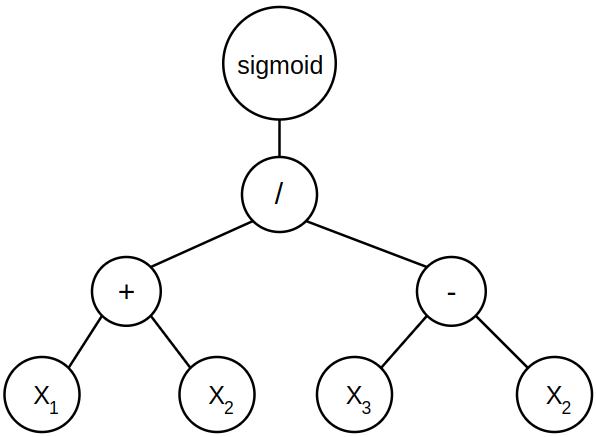
\includegraphics[scale=0.5]{Images/genotype_example.png}
	\caption{Представлення індивіду у вигляді дерева, який отримує на вхід три фічі: $X_1$, $X_2$, $X_3$ та обраховує наступну функцію, яка залежить від цих фіч - $sigmoid\left(\frac{X_1 + X_2}{X_3 - X_2}\right)$, де $sigmoid(x) = \frac{1}{1 + \exp(-x)}$}
	\label{fig_genotype}
\end{figure}

\section{Метрики оцінки якості моделей та функції втрат, для задач класифікації}


Існують різноманітні метрики для оцінювання якості моделі, наприклад точність (англ. accuracy)~\cite{ct6}, precision~\cite{ct6}, recall~\cite{ct7}, f1-score~\cite{ct8}. Формально ці метрики можна записати наступним чином (таблиця \ref{tab_metrics}).

\begin{table}[ht]
	\setfontsize{14pt}
	\caption{Формули основних метрик якості класифікаційних моделей}
	\label{tab_metrics}
	\centering
	\begin{tabular}{|c|c|}
		\hline
		Метрика & Формула \\
		\hline
		Accuracy & $\frac{TP + TN}{TP + TN + FP + FN}$ \\
		\hline
		Precision & $\frac{TP}{TP + FP}$ \\
		\hline
		Recall & $\frac{TP}{TP + FN}$ \\
		\hline
		F1-Score & $2 \times \frac{\text{Precision} \times \text{Recall}}{\text{Precision} + \text{Recall}}$ \\
		\hline
	\end{tabular}
\end{table}

Основна метрика, що використовується для загальної оцінки якості моделі, — це accuracy~\cite{ct6}. Ця метрика є найбільш інформативною, коли класи в даних розподілені рівномірно. Проте, в умовах сильного дизбалансу класів accuracy~\cite{ct6} може давати занадто оптимістичну картину ефективності моделі, оскільки вона враховує лише загальну кількість правильних передбачень.

Precision~\cite{ct6} краще використовувати, коли важливіше знизити кількість помилково позитивних результатів. Наприклад, у медичних тестах або в системах, де вартість помилки дуже висока.

Recall~\cite{ct7} є ключовою метрикою, коли важливо виявити всі можливі позитивні випадки. Це критично для ситуацій, де пропуск позитивних результатів може мати серйозні наслідки, наприклад, в системах раннього виявлення захворювань.

F1-score~\cite{ct8} використовується для оцінки балансу між precision~\cite{ct6} та recall~\cite{ct7}. Ця метрика особливо корисна, коли потрібно врахувати обидві ці характеристики одночасно, наприклад, у контексті інформаційного пошуку та класифікації текстів, де немає явної переваги між помилково позитивними та помилково негативними результатами.

Вибір метрики для конкретної задачі залежить від самої задачі, але гарною практикою є розрахунок одразу декількох метрик, для того, щоб бачити повну картину.

Функції втрат використовуються під час навчання моделей, щоб оптимізувати параметри моделі з метою мінімізації розбіжності між прогнозованими результатами та дійсними даними. Такі функції кількісно оцінюють помилки моделі та на основі значень такої функції оновлюються параметри моделі. Функцій втрат також існує велика кількість, але ми наведемо приклад двох функцій, одна з яких використовується для бінарної класифікації -- бінарна крос ентропія~\cite{ct27}, а інша для багатокласової класифікації -- крос ентропія~\cite{ct28}. Бінарна крос ентропія~\cite{ct27} та крос ентропія~\cite{ct28} виражаються наступними формулами:
\begin{equation}
	\label{eq:binary_cross_entropy}
	\text{binary cross entropy loss} = -\frac{1}{N} \sum_{i=1}^{N} \left( y_i \log(p_i) + (1 - y_i) \log(1 - p_i) \right)
\end{equation}
\begin{equation}
	\label{eq:cross_entropy}
	\text{cross entropy loss} = -\frac{1}{N} \sum_{i=1}^{N} \sum_{j=1}^{M} y_{ij} \log(p_{ij})
\end{equation}
де $N$ -- кількість спостережень у наборі даних, $M$ -- кількість можливих класів, $y_i$ -- фактична мітка класу для i-го спостереження, $y_{ij}$ -- бінарний індикатор, який показує чи належить $i$-те спостереження до класу $j$, $p_i$ -- прогнозована ймовірність, що спостереження $i$ належить до класу з міткою 1, $p_{ij}$ -- прогнозована ймовірність, що $i$-те спостереження належиить до класу $j$, $log$ -- натуральний логарифм.

\section{Процес навчання моделей для задач класифікації}


В цьому підрозділі ми розглянемо, як відбувається процес навчання MLP~\cite{ct26} та генетичного алгоритму.

Почнемо розгляд з  процесу навчання MLP~\cite{ct26}. Перед початком навчання ініціалізуються ваги мережі. Після того, як ваги були ініціалізовані, мережі подаються на вхід дані. Перший шар нейронів розраховує вихідний сигнал, де кожен нейрон розраховує його за формулою \ref{eq:neuron}, далі цей сигнал передається наступному шару, наступний шар розраховує вихідний сигнал, передає його далі і так це повторюється стільки разів, скільки в мережі шарів, останній шар розраховує вихідний сигнал, у випадку бінарної класифікації це буде одне значення для кожного вхідного прикладу з даних, яке буде відображати ймовірність того, що поточний приклад належить до класу 1, у випадку багатокласової класифікації, для кожного вхідного прикладу будуть розраховуватись $n$ - значень, де $n$ -- це кількість можливих класів, які будуть відображати ймовірність того, що поточний приклад належить до класу $i$. Після того, як були розраховані ймовірності належності прикладів до класу/класів, використовуючи значення цих ймовірностей розраховуються функції втрат за формулами \ref{eq:binary_cross_entropy}, \ref{eq:cross_entropy} для бінарної та багатокласової класифікації відповідно. Наступний крок є ключовим у навчанні MLP~\cite{ct26} -- зворотнє поширення помилки. Зворотнє поширення помилки полягає в обчисленні градієнтів функції втрат по відношенню до кожного вагового коефіцієнту в мережі, використовуючи правило ланцюгового диференціювання. Обчисленні градієнти використовуються для оновлення ваг у напрямку, що зменшує помилку (зазвичай за допомогою методу градієнтного спуску, або його варіантів, наприклад, Adam~\cite{ct9}). Описаний вище процес повторюється ітеративно певну кількість ітерацій, або поки не буде виконана умова завершення.

Тепер розглянемо процес навчання генетичного алгоритму. Першим кроком ініціалізується популяція (див. означення в переліку умовних позначень, скорочень і термінів) індивідів. Ініціалізація індивідів може відбуватися як повністю випадковим чином, так і з наперед заданими конкретними структурами індивідів. Для кожного індивіду в популяції розраховується фітнес-функція (див. означення в переліку умовних позначень, скорочень і термінів), яка вимірює як добре особина вирішує поставлену задачу. Для задач бінарної та багатокласової класифікації в якості фітнес функції використовуються формули \ref{eq:binary_cross_entropy} та \ref{eq:cross_entropy}, в цьому випадку, чим менше буде значення фітнес-функцій тим краще індивід буде пристосований до поточної задачі. Після того, як для кожного індивіду були розраховані фітнес-функції, за допомогою методу відбору обираються індивіди, які будуть брати участь у створені наступного покоління. Існує багато методів відбору, ось декілька прикладів: рулетковий відбір~\cite{ct2}, турнірний відбір~\cite{ct3} (випадковим чином обирається групка індивідів з усієї популяції і з цієї групки для репродукції обирається той індивід у якого найкраща фітнес функція), стабільний відбір (англ. Steady State Selection)~\cite{ct5}. Далі для генерації наступного покоління, до відібраних індивідів застосовується операція кросинговеру (див. означення в переліку умовних позначень, скорочень і термінів). Обрані індивіди розбиваються на пари і обмінюютьсся частинами своїх хромосом для створення нових індивідів. Цей процес є стохастичним, тобто які саме частини хромосом будуть обмінюватись визначається випадковим чином. До поширених методів кросинговеру відносяться одноточковий кросинговер~\cite{ct10} та багатоточковий кросинговер~\cite{ct11}. При одноточковому кросинговері~\cite{ct10} геноми обох батьків розділяються в одній випадково обраній точці, а потім їх сегменти обмінюються місцями. Багатоточковий кросинговер~\cite{ct11} включає декілька таких точок, що дозволяє формувати потомство з ще більшою генетичною різноманітністю. Після кросинговеру, гени нових особин можуть випадково змінюватись з певною, зазвичай низькою, ймовірністю -- цей процес називається мутацією (див. означення в переліку умовних позначень, скорочень і термінів). Мутація запобігає можливій стагнації всієї популяції в локальному оптимумі, вносячи нові варіанти в генетичний матеріал. Створені особини заміщують деякі, або всі особини в поточній популяції, в залежності від методу відбору. Описаний вище процес повторюється певну кількість поколінь, або поки не буде досягнуто задовільне значення фітнес-функції.

Важливим кроком під час навчання моделей є розділення даних на тренувальну та тестувальну вибірки. Тренувальна вибірка використовується для оновлення ваг моделі, у випадку MLP~\cite{ct26}, та генерацію нових поколінь, у випадку генетичного алгоритму. Градієнти, у випадку MLP~\cite{ct26}, розраховуються використовуючи значення функції втрат, яка була отримана в результаті роботи MLP~\cite{ct26}, який отримав на вході тренувальну вибірку. Фітнес-функції для індивідів, у випадку генетичного алгоритму, також розраховуються використовуючи тільки тренувальну вибірку. Тестувальна вибірка використовується для оцінки якості моделі під час навчання, для того, щоб можна було відслідковувати в який момент почнеться перенавчання (англ. overfit) і використовувати ті параметри моделі, які вона мала до початку перенавчання, це значно покращить узагальнювальну здатність моделей. Важливо зазначити, що тестувальна вибірка ніяким чином не впливає на оновлення параметрів моделей.

\section{Огляд суміжних робіт}

Як вже було описано в розділі \ref{sec:methods_of_solving_the_classification_problem} існують наступні методи вирішення задач класифікації: класичні статистичні методи, методи ML, методи глибинного навчання та генетичні алгоритми.

Статистичні методи добре підходять в тих випадках, коли нам важлива інтерпретованість результатів. Прикладом такого методу може бути логістична регресія~\cite{ct1}. Логістична регресія~\cite{ct1} -- це статистичний метод, який використовується для задачі бінарної класифікації. Метод базується на логістичній функції, яка оцінює ймовірності приналежності спостережень до однієї з двох категорій. Основною перевагою логістичної регресії~\cite{ct1} є її здатність працювати з даними, де таргетна зміна обмежена інтервалом [0,1], що робить її ідеальною для задач бінарної класифікації. Крім того, модель легко інтерпретувати, оскільки коефіцієнти моделі можуть бути представлені у вигляді шансів (англ. odds ratios). Застосування логістичної регресії~\cite{ct1} виявилося ефективним у багатьох областях, включаючи медицину для діагностики захворювань, в банківській справі для оцінки кредитного ризику, а також в соціальних науках для аналізу виборчих перегонів. Однією з найважливіших областей застосування статистичних методів у медицині є прогнозування серцево-судинних захворювань. Логістична регресія~\cite{ct1} часто використовується для аналізу ймовірності розвитку цих захворювань на основі різних ризикових факторів, таких як вік, кров'яний тиск, холестерин, куріння, сімейний анамнез та інші. В роботі Hosmer і Lemeshow~\cite{ct12}, метод логістичної регресії~\cite{ct1} було застосовано для визначення ймовірності настання серцевих нападів у пацієнтів на основі їхнього медичного анамнезу. Модель включала незалежні змінні, які були вибрані на основі клінічного досвіду та попередніх досліджень. Кожен з цих факторів був оцінений на його зв'язок з ризиком розвитку хвороби, і коефіцієнти моделі були інтерпретовані через шансові співвідношення, що дозволило медичним працівникам краще розуміти ризики. Зокрема, було встановлено, що високий кров'яний тиск та високий рівень холестерину значно підвищують шанси на розвиток серцевих захворювань, в той час як регулярні фізичні вправи та здоровий раціон харчування зменшують ці шанси. Ці висновки допомагають лікарям формулювати профілактичні рекомендації та лікувальні стратегії для пацієнтів з підвищеним ризиком. Такий підхід підкреслює значення логістичної регресії~\cite{ct1} не тільки як аналітичного інструменту, але й як засобу для підтримки клінічних рішень у медицині.

Методи ML, такі як k-найближчих сусідів~\cite{ct4} (англ. k-Nearest Neighbors, knn), залишаються одними з найпопулярніших через їхню простоту та ефективність у багатьох випадках. У статті Guo і співавторів~\cite{ct13} досліджено модифікований підхід до методу knn~\cite{ct4}, який використовується для класифікації даних у складних застосуваннях, таких як веб-майнінг. У цій статті автори фокусуються на застосуванні цього методу для класифікації великих наборів даних, де традиційні методи knn~\cite{ct4} часто зазнають труднощів через велику обчислювальну складність і залежність від вибору оптимального значення параметра \( k \). Автори пропонують новий метод -- kNNModel~\cite{ct13}, який автоматизує вибір \( k \) і використовує передбачувальну модель для підвищення ефективності класифікації. Цей підхід передбачає попереднє моделювання даних за допомогою визначення представників кожної класифікаційної категорії на основі тренувального набору даних. Представники, визначені методом, є центрами кластерів, що представляють групи схожих за характеристиками екземплярів. Свій підхід автори тестують на даних з репозиторію UCI. Використовуючи kNNModel~\cite{ct13}, автори провели експерименти, які показали значне покращення в точності класифікації порівняно зі стандартним методом knn~\cite{ct4}, особливо в умовах, де потрібно ефективно обробляти великі обсяги даних. Одним з ключових результатів експерименту є те, що застосування моделі kNNModel~\cite{ct13} дозволило значно скоротити час обчислень, необхідний для класифікації нових екземплярів, завдяки використанню попередньо підготовлених представників замість повторного обчислення відстаней до всіх точок даних.

Дослідження Soliman та Abd-elaziem~\cite{ct14} розглядає використання MLP~\cite{ct26} для спеціалізованої задачі класифікації зірок за їхніми спектральними характеристиками. MLP~\cite{ct26}, варіант нейронної мережі, є винятково підходящим для обробки нелінійних завдань, як-от аналіз астрофізичних даних, де потрібно розпізнавати складні взаємозв'язки між характеристиками. У цьому конкретному дослідженні використовувались дані з понад 100,000 спостережень, кожне з яких містить 18 ознак, таких як інтенсивність на різних довжинах хвиль. Ці особливості були використані для тренування MLP~\cite{ct26} з метою класифікації об'єктів на галактики та зорі. MLP~\cite{ct26}, яке було застосоване в дослідженні, містило кілька прихованих шарів, що дозволяло моделі ефективно вивчити складні патерни у даних. Ефективність класифікації, яку продемонструвала модель, склала 97$\%$. Такий високий показник точності підкреслює здатність MLP~\cite{ct26} ефективно обробляти великі обсяги складних даних та виділяти критично важливі особливості для розпізнавання патернів. Для оптимізації процесу тренування та досягнення максимальної точності було випробувано декілька оптимізаторів, серед яких Adagrad~\cite{ct29} показав найкращі результати з найвищою валідаційною точністю. Ці результати не тільки демонструють потенціал MLP~\cite{ct26} для вирішення астрофізичних задач класифікації, але й вказують на можливість його застосування в інших сферах, де потрібне швидке та ефективне рішення аналогічних задач. Завдяки такому дослідженню, можливо підвищити ефективність використання астрономічних даних та покращити розуміння структури та еволюції космосу.

Дослідження Robu та Holban~\cite{ct15} демонструє застосування генетичних алгоритмів у завданнях класифікації, де використовуються класичні набори даних: Car, Zoo та Mushrooms. В рамках цього дослідження автори впровадили новий підхід до фітнес-функцї, який враховує точність прогнозування та інтерпретованість правил. Фітнес-функція, запропонована в їхній роботі, включає в себе вагові коєфіцієнти, які дозволяють регулювати значимість точності прогнозування та інтерпретованості правиил. Це важливо, оскільки в генетичних алгоритмах не тільки важлива здатність правил точно класифікувати дані, але й можливість інтерпретувати ці правила. Такий підхід дозволяє створювати правила, які не тільки ефективні, але й інтерпретовані, що є критично важливим для застосувань, де необхідно пояснення моделі, наприклад, в медичних діагностиках чи у фінансовому секторі. Експериментальні результати, представлені в дослідженні, показали, що генетичні алгоритми можуть бути порівнянно ефективними з традиційними методами ML, такими як Наївний Баєс~\cite{ct16} та J48~\cite{ct17}, які також були застосовані до тих же даних. Це свідчить про великий потенціал генетичних алгоритмів в завданнях класифікації, особливо коли необхідно знайти баланс між точністю та інтерпретованістю результатів.

\chapconclude{\ref{chap:review}}

В цьому розділі було розглянуто теоретичні відомості про об'єкт та предмет дослідження, а саме про задачі бінарної та багатокласової класифікації та існуючі методи вирішення цих задач. Було здійснено короткиий огляд суміжних розділів, таких як класичні статистичні методи, методи ML, глибинне навчання та генетитичні алгоритми. Було оглянуто процеси навчання моделей, які вирішують задачі класифікації та метрики, що оцінюють якість роботи моделей.

Ми також вказали на важливості використання методів, які легко інтерпретувати та контролювати для сфер, де пояснення моделі є критично важливим.